\documentclass[11pt]{IEEEtran}

% ========================= Packages =========================
\usepackage{graphicx}
\usepackage{float}
\usepackage{pgfplots}
\usepackage{pgfplotstable}
\usepackage{csvsimple}
\usepackage{tikz}
\usepackage{circuitikz}
\usepackage{siunitx}
\usepackage{booktabs}
\usepackage{hyperref}
\usepackage{multirow}
\usepackage{tabularx}
\usepackage{nicematrix}
\usepackage{array}
%\usepackage{cite}
\pgfplotsset{compat=newest}

% ========================= Project Commands =========================
\newcommand{\comet}{C.O.M.E.T.}
\newcommand{\ares}{A.R.E.S.}
\newcommand{\phobos}{P.H.O.B.O.S.}
\newcommand{\deimos}{D.E.I.M.O.S.}
\newcommand{\insight}{INSIGHT}
\newcommand{\RHeight}{12}

% Existing IEEEtran class and Kyle's five-column booktabs formatting are retained.
% The narrower p{...} columns let prose fit on the page without overflowing.
\hypersetup{colorlinks=true,linkcolor=black,urlcolor=blue,citecolor=black}
\urlstyle{same}
\setlength{\emergencystretch}{3em}
\newcommand{\selecttech}[1]{\textbf{#1 (Selected)}}

% Replace figures/*.png with individual high-resolution functional block diagrams.
% Each diagram is intentionally a separate figure; absent files show a visible slot.
\newcommand{\fbdplaceholder}[2]{%
\IfFileExists{#1}{\includegraphics[width=0.97\linewidth,height=0.72\textheight,keepaspectratio]{#1}}{%
\fbox{\parbox[c][2.3in][c]{0.93\linewidth}{\centering\textbf{Functional Block Diagram Image Placeholder}\\[2mm]
#2\\[2mm]\texttt{\detokenize{#1}}\\[2mm]Place a separate exported diagram at this path before the final PDF submission.}}}}

\begin{document}
\onecolumn
%%%%%%%% Needs Project Title, Names of Team Members, Instructors, and Advisors %%%%%%%%%%%%%%%%%

\onecolumn

\newcommand{\Space}{\\[.5cm]}
%\lhead{A.U.R.O.R.A.}
%\chead {}
%\rhead{\comet}
\begin{center}
    \vfill
    \textbf{\Large AURORA Rocket and Experimental Systems (A.R.E.S.)}
\vfill
  \begin{figure}[h]
    \centering
    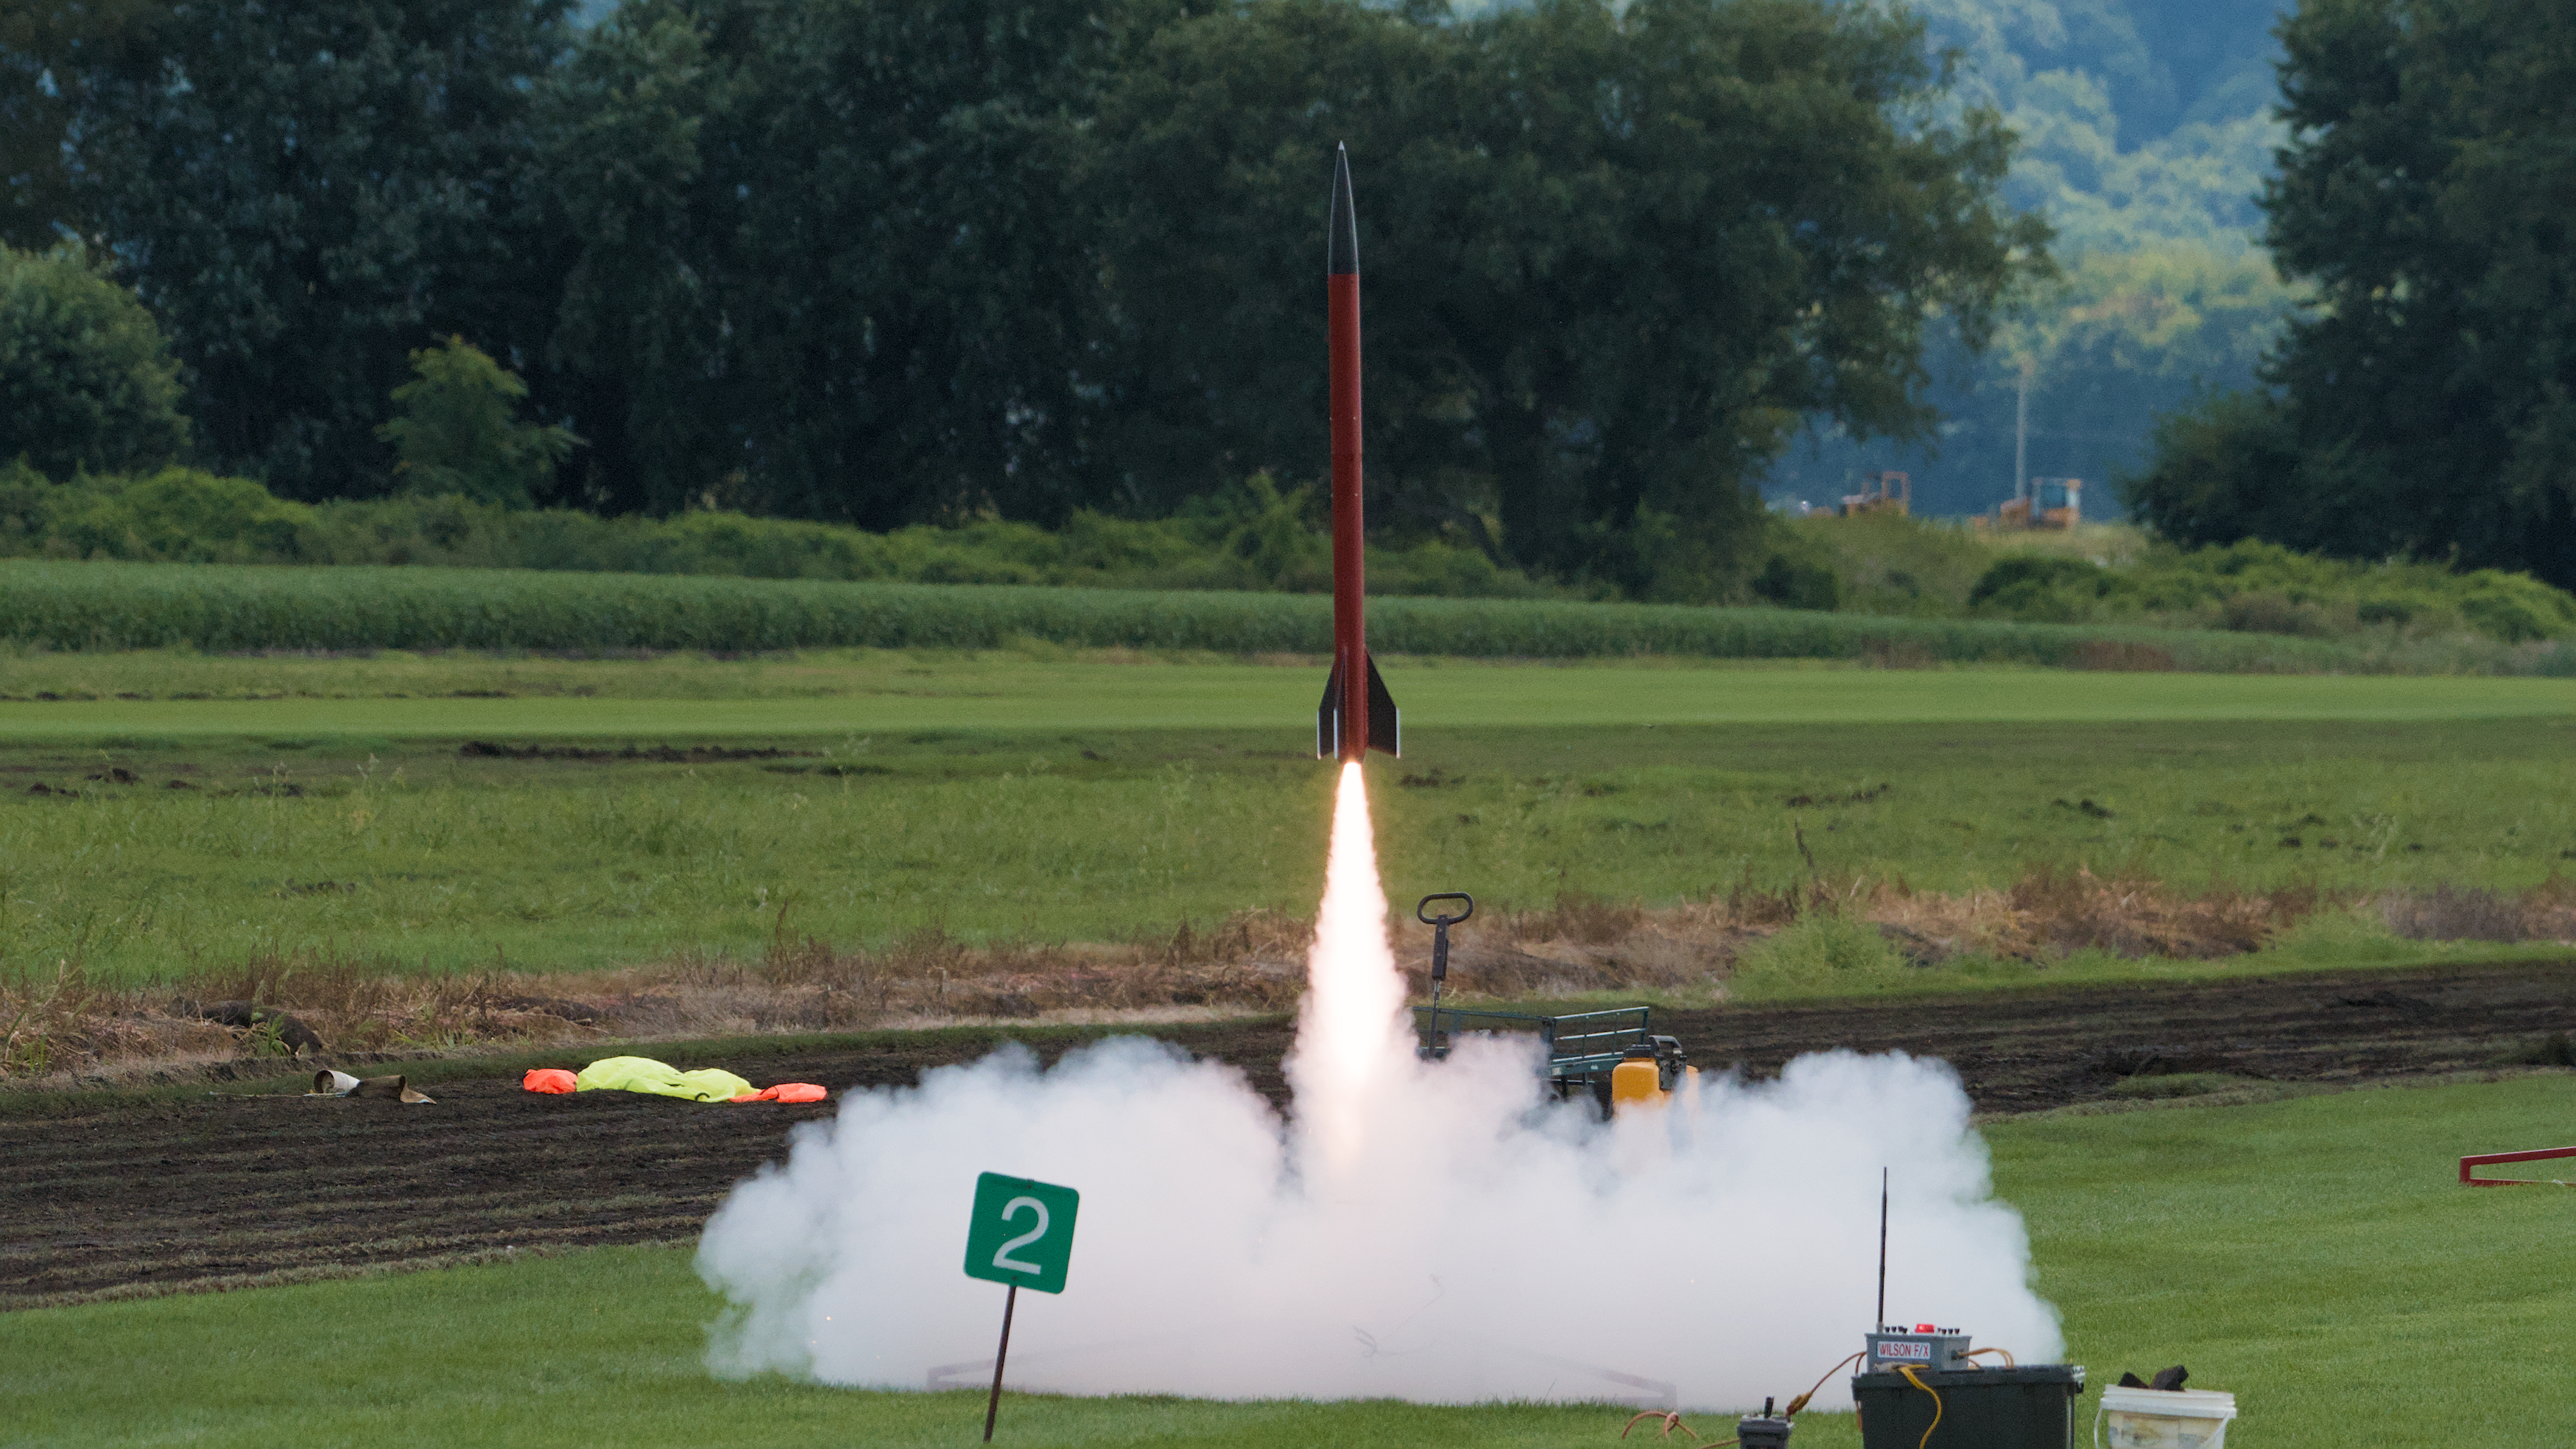
\includegraphics[trim={2cm 0 0 0}, clip,width=1\linewidth]{Documentation//ARES/Cover_Photo.jpg}
    \label{fig:placeholder}
\end{figure}
        

    \vfill
    \author[Kyle Eckert,
    \author[Nicholas Krupa,
    \author[Liam Gordon
    \vfill

    Technical Advisors\\Dr. Patricia Mellodge, Professor Allan Penda, Professor Loel Goldblatt \vfill
    Instructors\\Dr. Ying Yu, Dr. Xin Shen, Professor Jean Goulart\vfill
    \today

    \newpage
    
\end{center}

%\onecolumn
%\section{Project Team and Roles}

\begin{IEEEbiography}
[{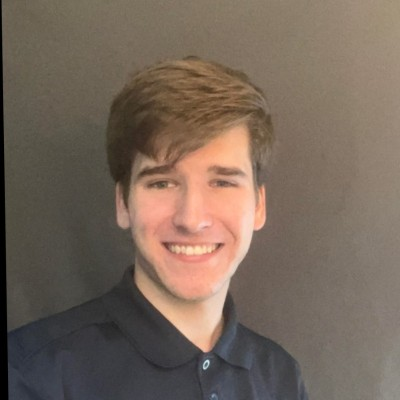
\includegraphics[width=1in,height=1.25in,clip,keepaspectratio]{Headshots/NHeadshot.jpg}}]
{\normalsize Nicholas Krupa}
\normalsize
is a senior electrical engineering major with minors in physics and mathematics. He is the founder and president of the AURORA Rocketry Team, a Senior Research Assistant within the Multiscale Metamaterial Research Laboratory, and holds a Level 2 High Power Rocketry certification through the National Association of Rocketry. He is a recipient of both a NASA Connecticut Space Grant Consortium Undergraduate Scholarship and an Undergraduate Research Grant for his work on phased-array antennas for satellite and space communication \cite{ctsgcSpring2024,ctsgcFall2024}. He is also a co-author of published research involving microwave metasurface design and characterization \cite{wells2024}. For this project, he will coordinate the overall \ares{} mission, including vehicle requirements, subsystem integration, flight operations, and development of the \deimos{} telemetry system and \comet{} flight computer. His previous experience includes leading the University of Hartford NASA RockSat-C team and developing several generations of custom high-power rocketry avionics. He completed an engineering internship with Ensign-Bickford Aerospace \& Defense (EBAD) during Summer 2026 and has accepted a full-time return offer with the company following graduation.
\end{IEEEbiography}

\begin{IEEEbiography}
[{
\includegraphics[width=1in,height=1.25in,clip,keepaspectratio]{Headshots/KHeadshot.jpg}}]
{\normalsize Kyle Eckert}

\normalsize
is a senior electrical engineering major with minors in audio engineering and mathematics and serves as the electrical lead for the Multiscale Metamaterial Research Laboratory. His work in the laboratory focuses on the design and development of experimental instrumentation for characterizing material properties at microwave frequencies. He also designs modifications to existing measurement systems to expand their operational and measurement capabilities. He was awarded a NASA Connecticut Space Grant Consortium Undergraduate Research Grant during the Spring 2026 award cycle for research involving rocket-based RF and metamaterial communication systems \cite{ctsgc2026}. Kyle was also the Lead Electrical Engineer and Flight Engineer with the 2026 RockSat program, where he designed and developed circuitry to enable experiments to fly aboard NASA sounding rockets and collect data under flight conditions. He holds a Level 1 High Power Rocketry certification and is a co-creator of the \comet{} dual-deployment system, a four-layer PCB-based avionics system. He will lead the design, fabrication, and testing of the \phobos{} phased-array antenna payload, with emphasis on RF electronics, antenna systems, and communication engineering.
\end{IEEEbiography}



\begin{IEEEbiography}
[{
\includegraphics[width=1in,height=1.25in,clip,keepaspectratio]{Headshots/LHeadshot.jpg}}]
{\normalsize Liam Gordon}
\normalsize
is a senior mechanical engineering major, president of the University of Hartford AIAA Student Chapter, and vice president of the AURORA Rocketry Team. He holds a Level 1 High Power Rocketry certification and has contributed to multiple student aerospace design and flight projects. His work on AURORA was recognized as one of the Top 3 Sophomore Projects at the University of Hartford's Spring 2025 CETA Design Expo \cite{uhartexpo2025}. He also participated in the University's inaugural AIAA Design/Build/Fly team, competing in Tucson, Arizona in 2025 \cite{uhartdbf2025}. Through the competition, he gained hands-on experience in aircraft design, CAD, fabrication, technical inspection, field testing, and rapid mechanical troubleshooting. He has additionally contributed to NASA Connecticut Space Grant-supported high-power rocketry work through AURORA. For the \ares{} project, he will lead vehicle mechanical design and manufacturing, including aerodynamic and structural analysis, CAD development, material selection, computational fluid dynamics, and finite element analysis. He will also oversee fabrication, mechanical integration, and structural verification of the completed vehicle.

\end{IEEEbiography}
\newpage


\tableofcontents
\newpage

\section{Use Case}
\subsection{Overview}
The AURORA Rocket and Experimental Systems (\ares{}) project is a student-developed, modular high-power sounding rocket being designed by the University of Hartford's AURORA rocketry team. Its immediate use case is participation in the 2027 International Rocket Engineering Competition (IREC), in the 10,000-foot commercial-off-the-shelf (COTS) propulsion category. The vehicle is intended to carry an experimental communications payload while providing the structural, avionics, and recovery functions needed to perform and document a safe research flight. The proposed vehicle is approximately \RHeight{}~ft long, 6~in in diameter, and constructed primarily from fiberglass. The mission target is 10,000~ft above ground level (AGL), not a demonstrated flight result. IREC eligibility, launch procedures, and payload integration will be checked against the applicable 2027 competition documents \cite{irecRules,irecGuide}.

Three student-developed electronic subsystems address different mission needs. \phobos{} is a scientific phased-array payload that evaluates directional communication and electronic beam steering from a translating and rotating rocket. \deimos{} is a nose-cone flight-instrumentation and telemetry module that measures position, pressure-derived altitude, acceleration, and vehicle attitude. \comet{} is a flight-event and dual parachute deployment controller that detects ascent and descent events, records measurements, and commands the drogue and main recovery parachute outputs. The broader \ares{} structure, propulsion section, harnesses, parachutes, and ground equipment connect these subsystems into a single mission.

Beyond its competition objectives, A.R.E.S. serves as an educational and research platform developed in collaboration with the University of Hartford's Multiscale Metamaterial Research Laboratory. This collaboration integrates the laboratory's ongoing research in microwave and metamaterial technologies into the P.H.O.B.O.S. phased-array antenna payload, extending laboratory-based research into a dynamic, real-world flight environment. By evaluating the performance of an electronically steered antenna aboard a sounding rocket, the project aims to advance research into directional communication systems for future aerospace applications. Consequently, mission success is defined not only by achieving the competition altitude target, but also by collecting meaningful RF and flight-performance data and safely recovering the vehicle and experimental hardware for postflight analysis and continued research.

\subsection{Practical Scenario}

The primary users of \ares{} are student engineers within the
University of Hartford's AURORA Rocketry Club and faculty
researchers seeking a reusable platform for testing experimental
avionics, communication systems, and aerospace technologies.
The project is developed in collaboration with the University's
Multiscale Metamaterial Research Laboratory, with the goal of
extending laboratory research in microwave and antenna
technologies into a realistic flight environment.

Development of the project is supported by Ensign-Bickford
Aerospace \& Defense (EBAD), which provides funding for the
rocket's development, and the NASA Connecticut Space Grant
Consortium, which funds development of the \phobos{} phased-array
antenna payload. Together, these efforts provide an opportunity
to demonstrate experimental communication technologies while
developing the infrastructure and experience necessary for
future student aerospace research.

A representative application of \ares{} is its participation
in the 2027 International Rocket Engineering Competition
(IREC) in Midland, Texas. The competition provides a
structured environment in which the team must design,
construct, test, and launch a sounding rocket targeting
an altitude of approximately 10,000~ft AGL while carrying
an experimental payload. This mission allows the team
to evaluate whether the developed systems can operate
reliably under the acceleration, vibration, rotation,
and environmental conditions experienced during flight.

Prior to launch, the team integrates the vehicle's electronic
subsystems, verifies electrical connections and battery
operation, and inspects the structural and recovery hardware.
The RF team evaluates antenna performance and communication
with the ground station, while the mechanical team verifies
the vehicle's structural interfaces, motor retention,
and recovery equipment. The recovery systems are checked
and armed according to the applicable range safety
procedures \cite{tripoliCode}.

During flight, \deimos{} measures and records the rocket's
position, acceleration, and orientation while transmitting
telemetry to the ground station. Simultaneously, \phobos{}
investigates electronically steered communication using a
2.4-GHz phased-array antenna. By adjusting the relative
phase of its antenna elements in response to the rocket's
orientation, the payload will attempt to maintain a
directional communication link with the receiving ground
station. The resulting measurements will allow researchers
to evaluate phased-array performance under dynamic flight
conditions rather than exclusively within a laboratory.

The \comet{} flight computer monitors onboard sensors
to identify flight events and initiate the dual-parachute
recovery sequence. The drogue parachute is commanded at
apogee, followed by the main parachute at a proposed
altitude of approximately 700~ft AGL. A separate commercial
deployment altimeter is also planned to provide an
independent recovery system.

Following landing, the team recovers the rocket and
downloads the recorded flight data. Measurements from
\deimos{} and \phobos{} are compared to investigate the
relationship between vehicle orientation, antenna steering,
and received signal performance. Flight data is also
compared against simulations to evaluate vehicle performance
and identify potential design improvements.

Success is therefore measured not only by achieving the
competition altitude target and safely recovering the
vehicle, but also by obtaining meaningful experimental
data that supports continued research within the
Multiscale Metamaterial Research Laboratory and future
development of the AURORA program.
\section{Requirements and Specifications}
The following values are \emph{design requirements or preliminary targets}, not claims of completed qualification. The planned verification methods are included so that the team can demonstrate compliance. Competition-imposed requirements remain subject to review of the current ESRA rules, design/test guide, and radio band plan \cite{irecRules,irecGuide,irecBand}.

\subsection{Vehicle Structure}
\begin{table}[H]
\centering\small
\begin{tabular}{@{}p{0.13\linewidth}p{0.20\linewidth}p{0.13\linewidth}p{0.08\linewidth}p{0.39\linewidth}@{}}
\toprule
\textbf{Category} & \textbf{Metric} & \textbf{Value} & \textbf{Unit} & \textbf{Notes}\\
\midrule
\multirow{5}{*}{Physical}
 & Body diameter & 6 & in & Fiberglass airframe; inspect dimensions.\\ \cmidrule{2-5}
 & Overall length & $\sim 12$ & ft & Final assembly measurement.\\ \cmidrule{2-5}
 & Airframe & G12 & --- & Fiberglass composite; inspect tubes and joints.\\ \cmidrule{2-5}
 & Nose profile & 5:1 & --- & Fiberglass ogive/Haack-style nose; verify fit.\\ \cmidrule{2-5}
 & Motor mount & 98 & mm & Commercial motor hardware with retention.\\
\midrule
\multirow{5}{*}{Flight}
 & Altitude target & 10,000 & ft AGL & IREC 10k COTS category; predict using final mass.\\ \cmidrule{2-5}
 & Static stability & $\geq 0.8$ & cal & Preliminary competition threshold; verify through flight envelope.\\ \cmidrule{2-5}
 & Launch guide & 1515 & rail & Planned 17-ft rail; verify geometry and availability.\\ \cmidrule{2-5}
 & Rail exit speed & $>25$ & m/s & Team design objective; verify with final motor simulation.\\ \cmidrule{2-5}
 & Flight loads & TBD & --- & Verify critical joints, fins, and payload mounts through FEA and tests.\\
\midrule
\multirow{3}{*}{Recovery}
 & Parachutes & 2 & --- & Drogue at apogee; main at planned $\sim700$ ft AGL.\\ \cmidrule{2-5}
 & Recovery computers & 2 & paths & Planned COTS and student-developed controllers.\\ \cmidrule{2-5}
 & Verification & Ground test & --- & Separation, extraction, continuity, harness, and attachment tests.\\
\bottomrule
\end{tabular}
\vspace{3mm}
\caption{\ares{} Vehicle and Mechanical Requirements}
\label{tab:ARES_Requirements_Table}
\end{table}

\subsection{Nose-Cone Tracking and Telemetry: \deimos{}}
\begin{table}[H]
\centering\small
\begin{tabular}{@{}p{0.13\linewidth}p{0.20\linewidth}p{0.13\linewidth}p{0.08\linewidth}p{0.39\linewidth}@{}}
\toprule
\textbf{Category} & \textbf{Metric} & \textbf{Value} & \textbf{Unit} & \textbf{Notes}\\
\midrule
\multirow{3}{*}{Physical}
 & Installation & Nose cone & --- & Fits 6-in, 5:1 nose and removable sled.\\ \cmidrule{2-5}
 & Assembly mass & $<200$ & g & Includes electronics and mounting; weigh assembly.\\ \cmidrule{2-5}
 & Antenna port & Right-angle SMA & --- & Mechanically supported, strain-relieved RF interface.\\
\midrule
\multirow{5}{*}{Functional}
 & Power source & Independent & --- & Battery powered; verify run time and brownout margin.\\ \cmidrule{2-5}
 & Position & GNSS & --- & Absolute location from GPS/GNSS receiver.\\ \cmidrule{2-5}
 & Motion & 3-axis + attitude & --- & Acceleration, angular motion, orientation estimate.\\ \cmidrule{2-5}
 & Pressure & Barometer & --- & Pressure-derived altitude and sensor logging.\\ \cmidrule{2-5}
 & Data storage & Onboard flash & --- & Preserve a full-flight record if radio link drops.\\
\midrule
\multirow{3}{*}{Performance}
 & Telemetry band & 915 & MHz & LoRa candidate; band-plan/FCC compliance review required.\\ \cmidrule{2-5}
 & Link range & $\geq4$ & km & Design target; demonstrate with range testing and link budget.\\ \cmidrule{2-5}
 & Log rate & 20 & Hz & Proposed design target; timestamp and verify sample data.\\
\bottomrule
\end{tabular}
\vspace{3mm}
\caption{\deimos{} Nose-Cone Tracking and Telemetry Requirements}
\label{tab:DEIMOS_Requirements_Table}
\end{table}

\subsection{Scientific Phased-Array Payload: \phobos{}}
\begin{table}[H]
\centering\small
\begin{tabular}{@{}p{0.13\linewidth}p{0.20\linewidth}p{0.13\linewidth}p{0.08\linewidth}p{0.39\linewidth}@{}}
\toprule
\textbf{Category} & \textbf{Metric} & \textbf{Value} & \textbf{Unit} & \textbf{Notes}\\
\midrule
\multirow{3}{*}{Physical}
 & Envelope & $\leq22$ & in & Must fit 6-in vehicle section; fit-check canister.\\ \cmidrule{2-5}
 & Payload mass & 2 & kg & Design allocation; confirm final IREC payload rule.\\ \cmidrule{2-5}
 & Board count & 2 & --- & Separate control/transceiver and RF antenna boards.\\
\midrule
\multirow{5}{*}{Functional}
 & Supply & 9 & V & Proposed battery input; characterize regulation losses.\\ \cmidrule{2-5}
 & Operating band & 2.4 & GHz & Preliminary selected ISM-band region.\\ \cmidrule{2-5}
 & Radiators & 2 panels of 4 & patches & Proposed two independent linear patch panels.\\ \cmidrule{2-5}
 & Steering & Phase controlled & --- & Independent phase shifts commanded using flight orientation.\\ \cmidrule{2-5}
 & RF interfaces & SMA/coax & --- & Secure RF connections; measure insertion loss and return loss.\\
\midrule
\multirow{3}{*}{Performance}
 & Link distance & $\sim2$ & km & Initial experiment target; assess 10k-ft mission link geometry.\\ \cmidrule{2-5}
 & Steering coverage & $\pm45$ & deg & Preliminary angular objective; verify measured beam pattern.\\ \cmidrule{2-5}
 & Radiated power & FCC-compliant & --- & Set by emission method, array gain, and applicable Part 15 rules; not automatically 1 W.\\
\bottomrule
\end{tabular}
\vspace{3mm}
\caption{\phobos{} Scientific Payload Requirements}
\label{tab:PHOBOS_Requirements_Table}
\end{table}

\subsection{Dual-Parachute Flight Computer: \comet{}}
\begin{table}[H]
\centering\small
\begin{tabular}{@{}p{0.13\linewidth}p{0.20\linewidth}p{0.13\linewidth}p{0.08\linewidth}p{0.39\linewidth}@{}}
\toprule
\textbf{Category} & \textbf{Metric} & \textbf{Value} & \textbf{Unit} & \textbf{Notes}\\
\midrule
\multirow{4}{*}{Physical}
 & PCB envelope & $\sim2.5\times1$ & in & Compact board objective; confirm hardware layout.\\ \cmidrule{2-5}
 & Power & Dedicated & --- & Battery and regulator; qualify full electrical load.\\ \cmidrule{2-5}
 & Storage & 128 & Mbit & Proposed nonvolatile flash capacity.\\ \cmidrule{2-5}
 & Arming & External & --- & Safe arm/disarm access without opening vehicle.\\
\midrule
\multirow{5}{*}{Functional}
 & Sensors & Baro + IMU & --- & Independent flight phase measurements.\\ \cmidrule{2-5}
 & Deployment outputs & 2 & channels & Electrically qualified main and drogue outputs.\\ \cmidrule{2-5}
 & Continuity & Monitored & --- & Indicate channel condition before launch.\\ \cmidrule{2-5}
 & User feedback & Audible/status & --- & Speaker and indicators; USB-C configuration/log access.\\ \cmidrule{2-5}
 & Backup controller & COTS & --- & Independent altimeter planned for recovery redundancy.\\
\midrule
\multirow{3}{*}{Performance}
 & Launch detection & 3g or 150 ft & --- & Candidate thresholds; verify in software tests.\\ \cmidrule{2-5}
 & Drogue command & Apogee & --- & Verify with simulated pressure/acceleration profiles.\\ \cmidrule{2-5}
 & Main command & $\sim700$ & ft AGL & Proposed main deployment setting; verify with ground tests.\\
\bottomrule
\end{tabular}
\vspace{3mm}
\caption{\comet{} Dual-Deployment Computer Requirements}
\label{tab:COMET_Requirements_Table}
\end{table}

\subsection{Applicable Standards and Ethical Design Considerations}
The proposed high-power flight requires compliance with 14 CFR Part 101 Subpart C, appropriate airspace coordination, the launch organizer's range rules, and the 2027 IREC documentation \cite{faaRockets,irecRules,irecGuide}. The Tripoli Unified Safety Code and NFPA 1127 provide high-power rocketry safety guidance for certified motors, recovery hardware, arming, and launch operations \cite{tripoliCode,nfpa1127}. Custom PCBs will use IPC-2221 and IPC-A-610 as design and workmanship references.

Radio-system authorization must be assessed separately for each transmitter. In particular, a 2.4-GHz phased array cannot assume that a generic ``$<1$ W'' figure establishes compliance: the applicable emission rule, occupied bandwidth, conducted power, directional antenna gain, and aggregate array output all matter under 47 CFR $\S$15.247 \cite{fcc15247}. Any amateur-radio operation under Part 97 requires separate licensing and operating-rule review \cite{fcc97113}. The final student frequency plan must also comply with the IREC event band plan \cite{irecBand}. The project uses pyrotechnic deployment hardware; all handling and testing must be conducted using qualified supervision, electrically inhibited circuits, documented checklists, and appropriate range approval. Nothing in this draft constitutes flight authorization.

\section{System Functional Block Diagrams}

\subsection{\phobos{} Phased-Array Antenna System}
%The functional paths are battery $\rightarrow$ power regulation $\rightarrow$ RP2040 control/transceiver, followed by RF synthesis and power distribution $\rightarrow$ phase shifters $\rightarrow$ SMA connections $\rightarrow$ patch antennas. The control MCU receives orientation information, updates phase settings, monitors system status, and logs flight-experiment data. Electrical power, digital control, and RF paths must remain distinguishable in the diagram.
\begin{figure}[H]
    \centering
    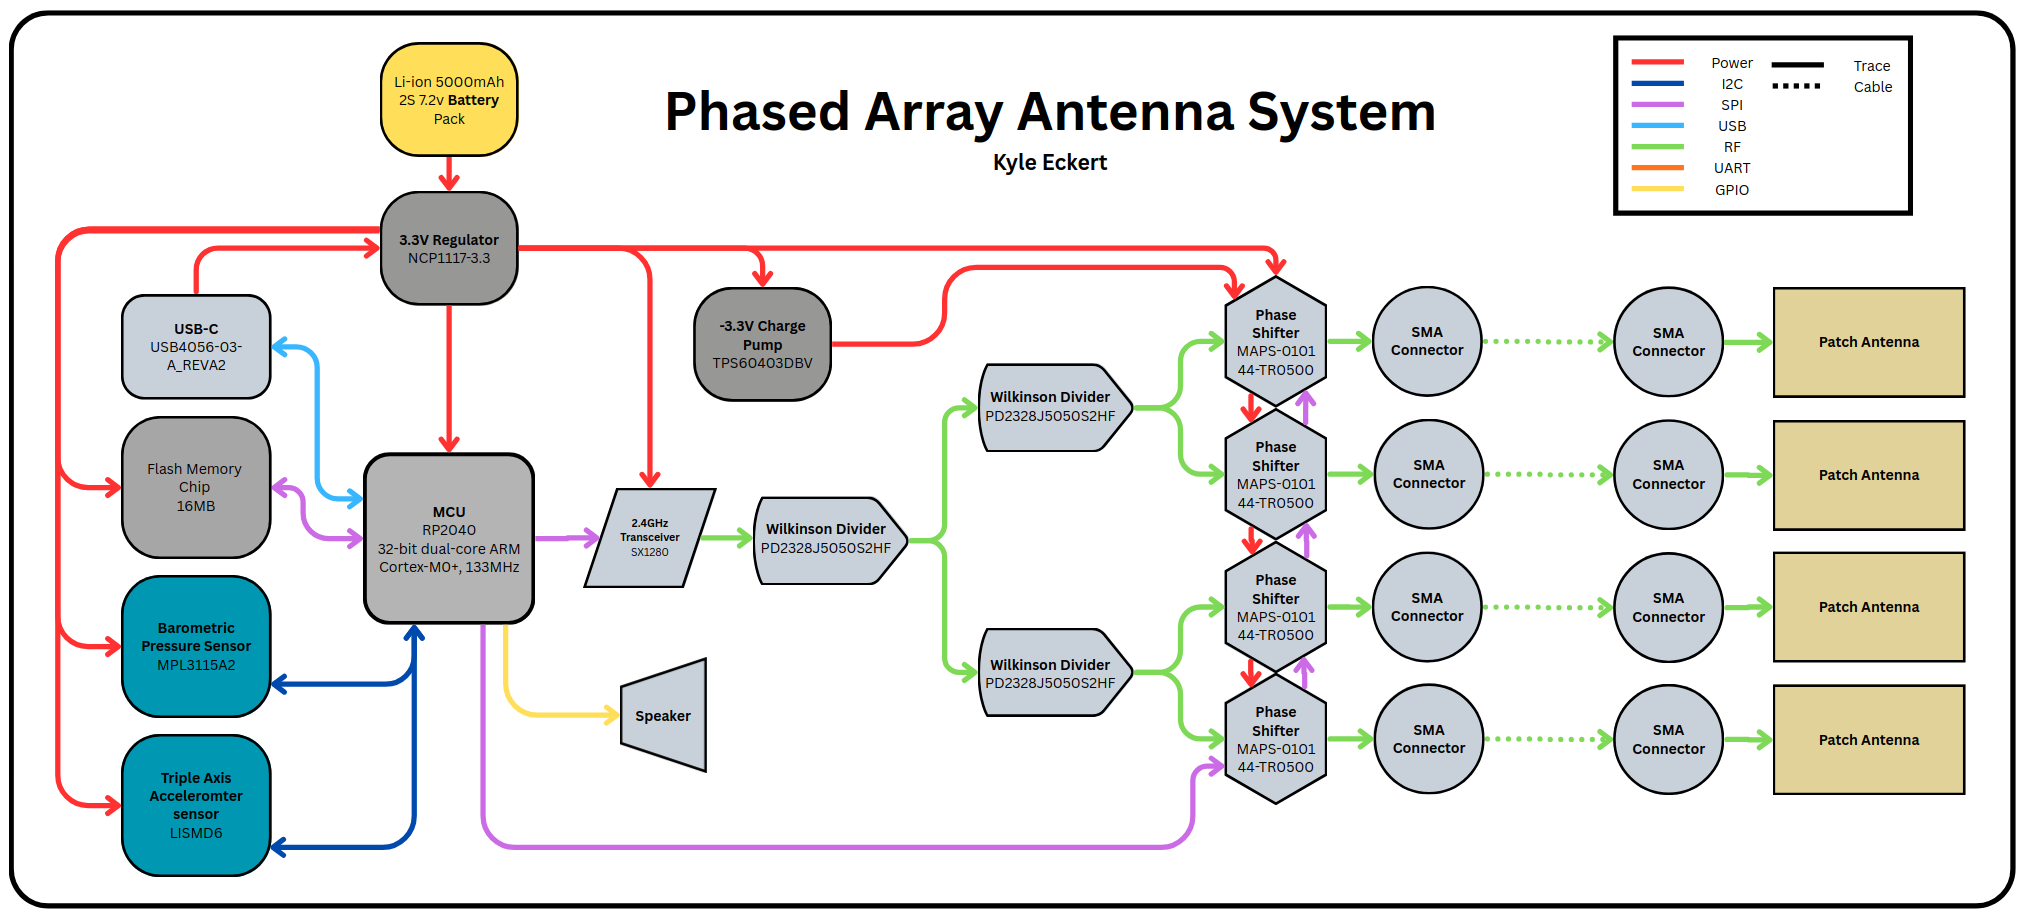
\includegraphics[width=.75\linewidth]{Documentation/Pics/PAA_Block_Diagram.png}
    \caption{\phobos{} Phased array antenna functional block diagram}
    \label{fig:PAA_Block}
\end{figure}

\subsection{\deimos{} Nose-Cone Tracking System}
\begin{figure}[H]
    \centering
    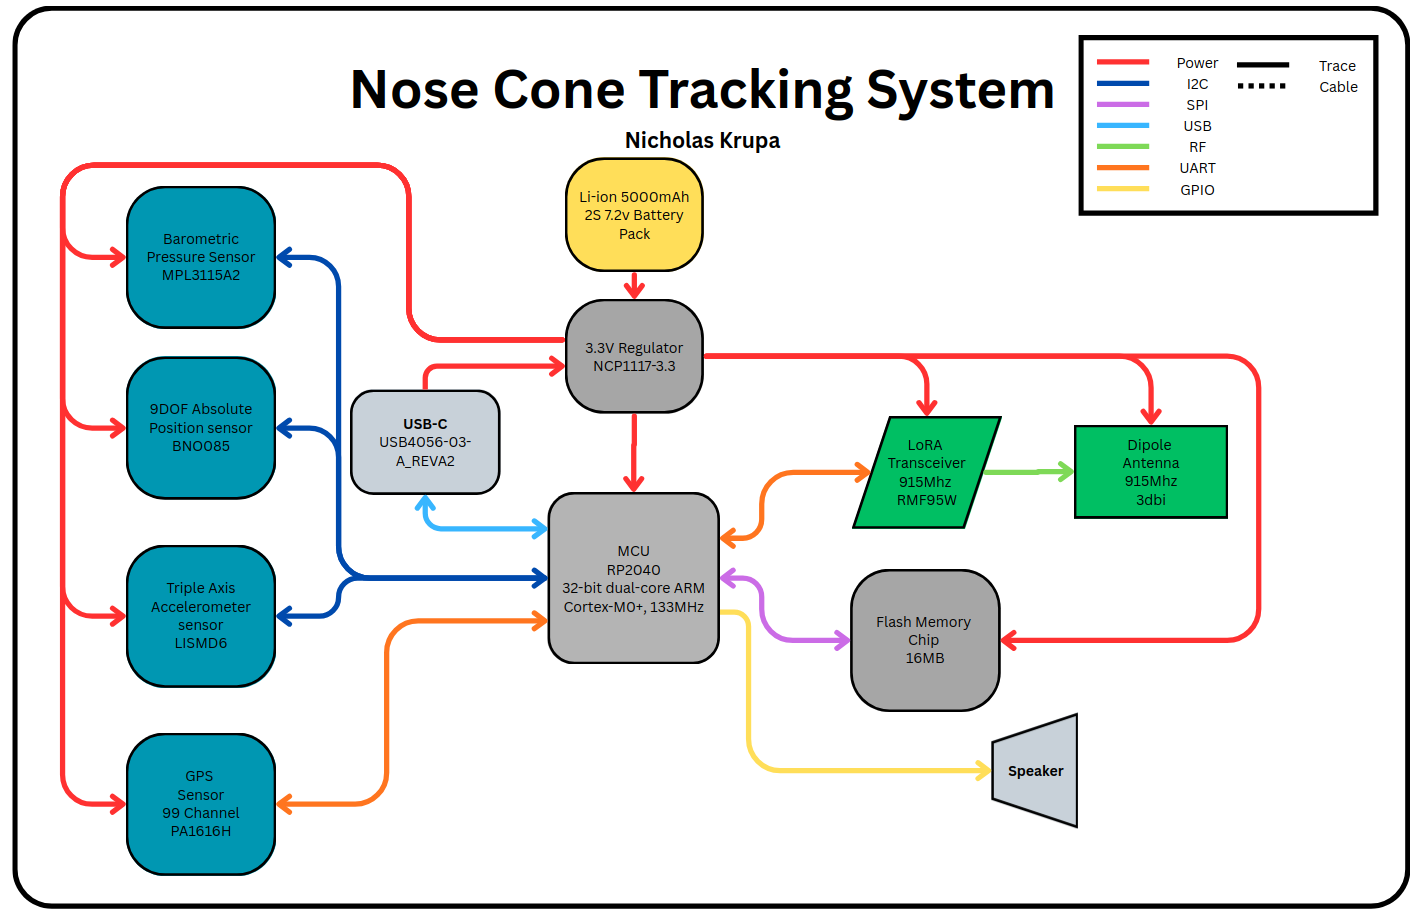
\includegraphics[width=.75\linewidth]{Documentation/Pics/NC_Block_Diagram.png}
    \caption{\deimos{} Nose cone telemetry functional block diagram}
    \label{fig:NC_Block}
\end{figure}

\subsection{\comet{} Dual-Parachute Deployment System}
\begin{figure}[H]
    \centering
    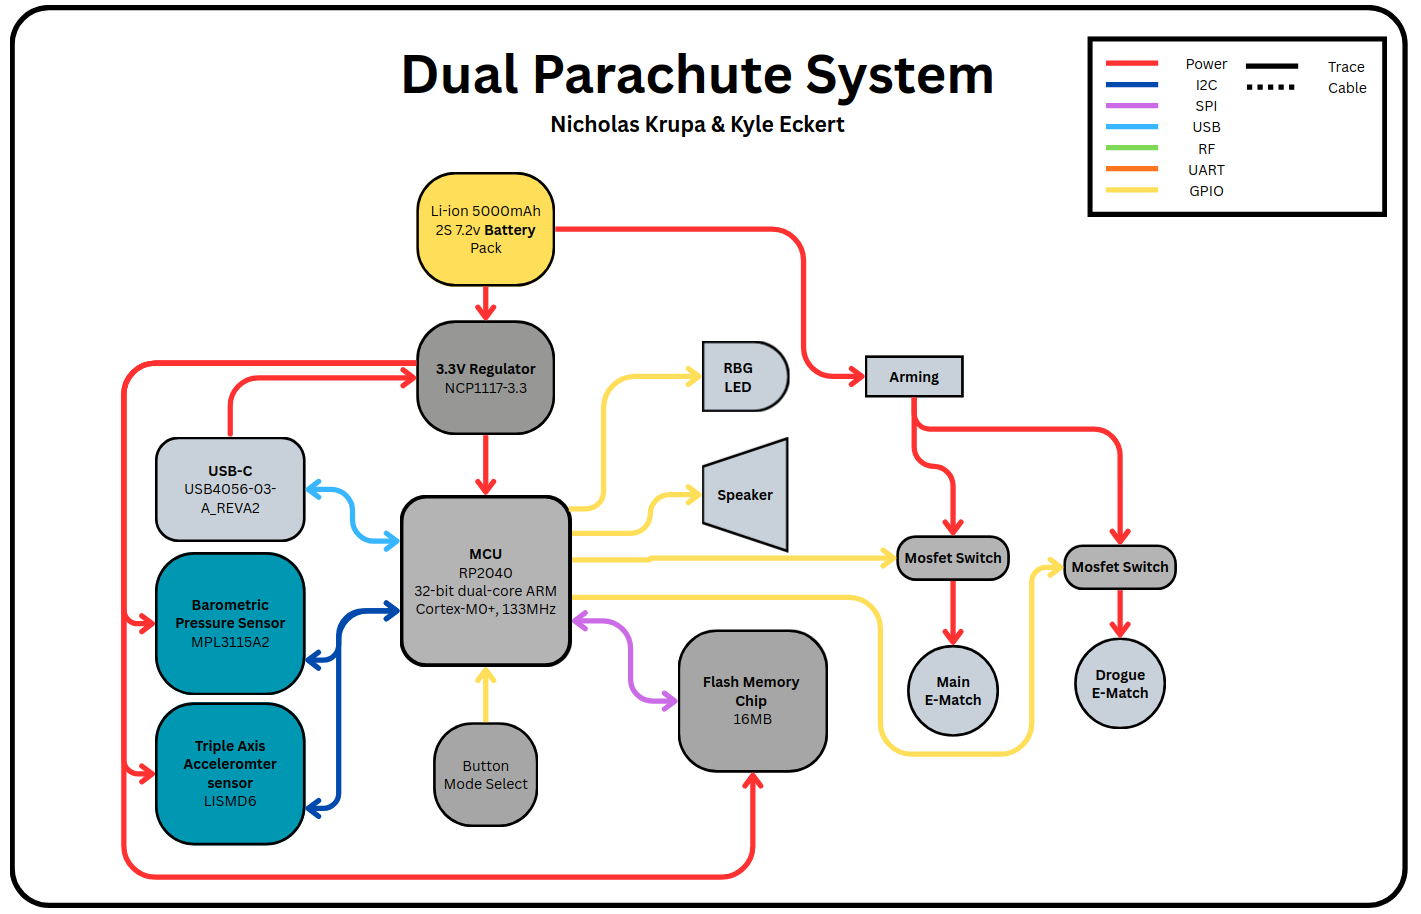
\includegraphics[width=.75\linewidth]{Documentation/Pics/DPS_Block_Diagram.png}
    \caption{\comet{} dual parachute deployment control functional block diagram}
    \label{fig:DPS_Block}
\end{figure}

\subsection{Nicholas Krupa - Electrical Engineering}

\subsubsection{Microcontroller Selection}
The microcontroller must interface with multiple sensors, manage data logging, and control peripheral devices within a compact, battery-powered flight computer. The RP2040 was selected because its 7~mm $\times$ 7~mm package, two processor cores, and flexible SPI, I\textsuperscript{2}C, UART, USB, and programmable I/O interfaces meet these needs without excessive cost or PCB area. Raspberry Pi also provides extensive hardware design documentation and software support. Unlike the ESP32-S3, the RP2040 has no integrated Wi-Fi or Bluetooth transmitter; using a separate radio module allows the team to control its operating band and reduces unnecessary onboard RF hardware near the 2.4-GHz experiment. Most importantly, previous AURORA hardware and firmware already use the RP2040, reducing development time and integration risk \cite{rp2040,stm32,esp32}.

\begin{table}[H]
\centering\small
\begin{tabular}{@{}p{0.11\linewidth}p{0.14\linewidth}p{0.215\linewidth}p{0.215\linewidth}p{0.215\linewidth}@{}}
\toprule
\textbf{Category} & \textbf{Feature} & \textbf{RP2040 (Selected)} & \textbf{STM32L432} & \textbf{ESP32-S3} \\
\midrule
\multirow{4}{*}{MCU}
 & Size / cost & 7$\times$7-mm QFN; low-cost chip and compact PCB layout. & Compact, low-power MCU; part and development costs depend on variant. & Capable MCU; wireless functionality adds design considerations. \\ \cmidrule{2-5}
 & Interfaces & Two SPI, two I\textsuperscript{2}C, two UART, USB, and eight PIO state machines. & Strong interfaces and integrated hardware floating-point unit. & Extensive peripherals and higher processing capability. \\ \cmidrule{2-5}
 & Onboard radio & No Wi-Fi/Bluetooth; RF communication remains on selected external modules. & No integrated Wi-Fi/Bluetooth; also requires an external radio. & Integrated 2.4-GHz Wi-Fi/Bluetooth; can be disabled if unused. \\ \cmidrule{2-5}
 & Development & Extensive documentation, existing team PCBs and reusable firmware. & New PCB and firmware development would be required. & New PCB and firmware development would be required. \\
\bottomrule
\end{tabular}
\vspace{3mm}
\caption{Microcontroller comparison based on integration, cost, and development risk.}
\label{tab:MCU_Comparison}
\end{table}

\noindent\textbf{Selection rationale:} The RP2040 offers sufficient processing and I/O for the required tasks without adding a wireless subsystem that the project does not need. Its main tradeoffs are the lack of a hardware floating-point unit and the need for external flash and RF hardware; these are acceptable given the team's prior experience.

\subsubsection{Barometric Sensor Selection}
Barometric measurements provide altitude information for flight analysis and event detection. The MPL3115A2 was selected because its 20--110~kPa \emph{operating} pressure range and 50--110~kPa \emph{calibrated} range include the pressures expected during a 10,000-ft flight. Its stated altitude-output range is approximately $-698$ to 11,775~m. In low-oversampling, one-shot operation, the datasheet specifies a minimum conversion interval of 6~ms at $1\times$ oversampling, or 34~ms at $8\times$ oversampling, enabling relatively fast sampling when configured appropriately.\cite{mpl,bmp390,bmp581}.

\begin{table}[H]
\centering\small
\begin{tabular}{@{}p{0.11\linewidth}p{0.14\linewidth}p{0.215\linewidth}p{0.215\linewidth}p{0.215\linewidth}@{}}
\toprule
\textbf{Category} & \textbf{Feature} & \textbf{MPL3115A2 (Selected)} & \textbf{BMP390} & \textbf{BMP581} \\
\midrule
\multirow{4}{*}{Pressure}
 & Range & 20--110~kPa operating; 50--110~kPa calibrated. & 30--125~kPa full-accuracy range. & 30--125~kPa full-accuracy range. \\ \cmidrule{2-5}
 & Sampling & 6-ms minimum at $1\times$ oversampling in one-shot mode; slower at higher oversampling. & Up to 200-Hz sampling; faster maximum rate. & Up to 480-Hz sampling; fastest of the three. \\ \cmidrule{2-5}
 & Interface & I\textsuperscript{2}C, internal compensation, direct altitude output. & I\textsuperscript{2}C/SPI; host computes altitude. & I\textsuperscript{2}C/SPI/I3C; host computes altitude. \\ \cmidrule{2-5}
 & Availability / use & Active product with distributor stock; already used by AURORA. & Available newer alternative; new integration and tests. & Available newer alternative; new integration and tests. \\
\bottomrule
\end{tabular}
\vspace{3mm}
\caption{Barometric sensor comparison emphasizing usable range, sampling, and availability.}
\label{tab:Pressure_Comparison}
\end{table}

\noindent\textbf{Selection rationale:} Although the Bosch alternatives support higher maximum sample rates, the MPL3115A2 provides sufficient pressure range and configurable measurement timing for the proposed mission while allowing existing circuitry and software to be reused.

\subsubsection{Telemetry Radio Selection}
The nose-cone telemetry link must be reliable and serviceable without requiring the team to design a radio transceiver from discrete RF components. The RFM95W was selected as a purchasable 868/915-MHz LoRa module with an established SPI interface and prior use in AURORA telemetry hardware. This allows the team to retain existing radio drivers, ground-station equipment, and packet configuration rather than introduce an untested chip-level RF design. It also exposes an \texttt{ANT} pad that can be routed on the host PCB to a rigid, right-angle SMA connector, avoiding an internal U.FL-only antenna connection. The SMA connector is \emph{not} built into the RFM95W module; the host-board RF trace, impedance matching, and connector mounting still require engineering and testing \cite{rfm95,sx1262,sx1280}.

\begin{table}[H]
\centering\small
\begin{tabular}{@{}p{0.11\linewidth}p{0.14\linewidth}p{0.215\linewidth}p{0.215\linewidth}p{0.215\linewidth}@{}}
\toprule
\textbf{Category} & \textbf{Feature} & \textbf{RFM95W (Selected)} & \textbf{SX1262 (IC)} & \textbf{SX1280 (IC)} \\
\midrule
\multirow{4}{*}{Telemetry}
 & Integration & Purchasable 16$\times$16-mm RF module; less RF circuitry to design. & Bare transceiver needs RF network or a separate module design. & Bare transceiver needs RF network or a separate module design. \\ \cmidrule{2-5}
 & Antenna path & \texttt{ANT} pad can feed a PCB-mounted right-angle SMA connector. & External antenna possible with suitable RF layout. & External antenna possible with suitable RF layout. \\ \cmidrule{2-5}
 & Previous systems & Reuses established AURORA driver, packet format, and receiver setup. & New driver and PCB; air-interface compatibility must be verified. & New driver and 2.4-GHz ground station required. \\ \cmidrule{2-5}
 & Flight link & 915-MHz LoRa candidate; previously tested by team; range still needs validation. & Efficient newer sub-GHz option; additional qualification required. & Higher-rate 2.4-GHz option; overlaps payload spectrum. \\
\bottomrule
\end{tabular}
\vspace{3mm}
\caption{LoRa radio comparison emphasizing module integration and system compatibility.}
\label{tab:Radio_Comparison}
\end{table}

\noindent\textbf{Selection rationale:} The RFM95W was selected for its backward compatibility with AURORA's previous telemetry systems, which utilized Adafruit's socketed LoRa modules. Its availability and established software support simplify integration, while the module's antenna pad allows RF routing to a full-size, board-mounted SMA connector for improved mechanical rigidity and reliability during flight.

\noindent\textbf{Overall selected approach:} RP2040 processing, MPL3115A2 barometry, complementary inertial sensing, and RFM95W telemetry with a board-mounted SMA antenna interface. These selections prioritize compact integration, well-documented components, cost, and reuse of proven team designs.


\subsection{Kyle Eckert - Electrical Engineering}
\subsubsection{Phased-Array Operating Frequency}
In a phased array, changing the phase of the signal at each antenna element steers the direction of constructive interference. Frequency affects the size and spacing of the patches, free-space path loss, and the available RF components. The team compared 915 MHz, 2.4 GHz, and 5 GHz as candidates. The 2.4-GHz band was chosen as the best packaging and implementation compromise for a six-inch rocket \cite{phased,fcc15247}.

\begin{table}[H]
\centering\small
\begin{tabular}{@{}p{0.115\linewidth}p{0.145\linewidth}p{0.21\linewidth}p{0.21\linewidth}p{0.21\linewidth}@{}}
\toprule
\textbf{Category} & \textbf{Feature} & \textbf{915 MHz} & \textbf{2.4 GHz (Selected)} & \textbf{5 GHz} \\
\midrule
\multirow{4}{*}{RF band}
 & Antenna size & Con: Large elements and spacing. & Pro: Patch sizes fit the available vehicle space. & Pro: Smaller elements and spacing. \\ \cmidrule{2-5}
 & Free-space loss & Pro: Lowest loss of the three at equal distance and gains. & Moderate loss compared with alternatives. & Con: Highest loss of the three at equal gains. \\ \cmidrule{2-5}
 & RF hardware & Pro: Common telemetry parts. Con: Large array geometry. & Pro: Broad availability of RF components. & Con: Increased fabrication and integration demands. \\ \cmidrule{2-5}
 & Overall fit & Con: Difficult array packaging. & Pro: Suitable balance of aperture and complexity. & Con: Less favorable development tradeoff. \\
\bottomrule
\end{tabular}
\vspace{3mm}
\caption{Phased-array frequency comparison (Kyle Eckert).}
\label{tab:Frequency_Comparison}
\end{table}

\subsubsection{RF Architecture and Phase Control}
A phased array requires a method of dividing the transmitted signal and controlling the phase at each patch. Digital phase shifters are preferred for repeatable MCU-controlled settings. Packaged power dividers and coaxial feeds reduce the amount of custom microwave layout required for an initial flight prototype, although their losses and phase errors still need measurement \cite{phased,wilkinson,rfLaminate}.

\begin{table}[H]
\centering\small
\begin{tabular}{@{}p{0.125\linewidth}p{0.18\linewidth}p{0.22\linewidth}p{0.22\linewidth}p{0.14\linewidth}@{}}
\toprule
\textbf{Category} & \textbf{Technology} & \textbf{Pros} & \textbf{Cons} & \textbf{Decision} \\
\midrule
\multirow{2}{*}{Phase control}
 & Analog shifter & Continuous adjustment. & Bias and calibration complexity. & Alternate \\ \cmidrule{2-5}
 & \textbf{Digital shifter} & Repeatable, MCU-commanded phase settings. & Finite phase resolution. & \textbf{Selected} \\
\midrule
\multirow{2}{*}{RF divider}
 & Printed Wilkinson & Direct PCB integration. & RF layout and EM verification required. & Alternate \\ \cmidrule{2-5}
 & \textbf{Packaged splitter} & Characterized component for a first prototype. & Insertion loss and component availability. & \textbf{Selected} \\
\midrule
\multirow{2}{*}{Patch feed}
 & Microstrip feed & Compact, planar construction. & Tight matching and layout tolerances. & Alternate \\ \cmidrule{2-5}
 & \textbf{Coaxial feed} & Flexible routing and familiar connectors. & Cable/connector loss and mechanical strain. & \textbf{Selected} \\
\bottomrule
\end{tabular}
\vspace{3mm}
\caption{Phased-array RF architecture comparison (Kyle Eckert).}
\label{tab:RF_Comparison}
\end{table}

\noindent\textbf{Selected approach:} A 2.4-GHz array with separate control and RF boards, digitally controlled phase shifters, packaged dividers, and coax-fed patches. Vector-network-analyzer, beam-pattern, link-range, and regulatory testing will be needed before claiming flight-ready performance.


\section{Literature Search: Source List}
\begingroup\small
\begin{thebibliography}{99}
\bibitem{irecRules} Experimental Sounding Rocket Association, ``2027 IREC Rules \& Requirements, REV P1,'' 2026. [Online]. Available: \url{https://www.esrarocket.org/documents-and-forms}
\bibitem{irecGuide} Experimental Sounding Rocket Association, ``2027 IREC Design, Test and Evaluation Guide, REV P1,'' 2026. [Online]. Available: \url{https://www.esrarocket.org/documents-and-forms}
\bibitem{irecBand} Experimental Sounding Rocket Association, ``IREC Student Band Plan (2026 revision; 2027 update pending),'' [Online]. Available: \url{https://www.esrarocket.org/documents-and-forms}
\bibitem{faaRockets} Federal Aviation Administration, ``Amateur Rockets: 14 CFR Part 101, Subpart C,'' [Online]. Available: \url{https://www.faa.gov/space/licenses/amateur-rockets}
\bibitem{tripoliCode} Tripoli Rocketry Association, ``Tripoli Unified Safety Code,'' ver. 2, effective January 2026. [Online]. Available: \url{https://www.tripoli.org/safetycode}
\bibitem{nfpa1127} National Fire Protection Association, ``NFPA 1127: Code for High Power Rocketry,'' 2026 ed. [Online]. Available: \url{https://webstore.ansi.org/standards/nfpa/nfpa11272026}
\bibitem{fcc15247} Federal Communications Commission, ``47 CFR $\S$15.247: Operation within the bands 902--928 MHz, 2400--2483.5 MHz, and 5725--5850 MHz.'' [Online]. Available: \url{https://www.ecfr.gov/current/title-47/section-15.247}
\bibitem{fcc97113} Federal Communications Commission, ``47 CFR $\S$97.113: Prohibited transmissions.'' [Online]. Available: \url{https://www.ecfr.gov/current/title-47/section-97.113}
\bibitem{rp2040} Raspberry Pi, ``RP2040 Specifications.'' [Online]. Available: \url{https://www.raspberrypi.com/products/rp2040/specifications/}
\bibitem{stm32} STMicroelectronics, ``STM32L432KC: Ultra-Low-Power Arm Cortex-M4 with FPU.'' [Online]. Available: \url{https://www.st.com/en/microcontrollers-microprocessors/stm32l432kc.html}
\bibitem{esp32} Espressif Systems, ``ESP32-S3 Wi-Fi and Bluetooth LE SoC.'' [Online]. Available: \url{https://www.espressif.com/en/products/socs/esp32-s3}
\bibitem{mpl} NXP Semiconductors, ``MPL3115A2 Pressure Sensor / Altimeter Data Sheet.'' [Online]. Available: \url{https://www.nxp.com/docs/en/data-sheet/MPL3115A2.pdf}
\bibitem{bmp390} Bosch Sensortec, ``BMP390 Pressure Sensor.'' [Online]. Available: \url{https://www.bosch-sensortec.com/en/products/environmental-sensors/pressure-sensors/bmp390}
\bibitem{bmp581} Bosch Sensortec, ``BMP581 Pressure Sensor.'' [Online]. Available: \url{https://www.bosch-sensortec.com/en/products/environmental-sensors/pressure-sensors/bmp581}
\bibitem{bno085} CEVA, ``BNO08X Family Data Sheet.'' [Online]. Available: \url{https://www.ceva-ip.com/wp-content/uploads/BNO080_085-Datasheet.pdf}
\bibitem{lsm} STMicroelectronics, ``LSM6DSO Six-Axis Inertial Module.'' [Online]. Available: \url{https://www.st.com/en/mems-and-sensors/lsm6dso.html}
\bibitem{adxl} Analog Devices, ``ADXL375: 3-Axis, $\pm200$ g Digital MEMS Accelerometer.'' [Online]. Available: \url{https://www.analog.com/en/products/adxl375.html}
\bibitem{h3lis} STMicroelectronics, ``H3LIS331DL High-g Digital Accelerometer.'' [Online]. Available: \url{https://www.st.com/en/mems-and-sensors/h3lis331dl.html}
\bibitem{rfm95} HopeRF, ``RFM95W LoRa Module.'' [Online]. Available: \url{https://www.hoperf.com/modules/lora/RFM95W.html}
\bibitem{sx1262} Semtech, ``SX1262 LoRa Connect Transceiver.'' [Online]. Available: \url{https://www.semtech.com/products/wireless-rf/lora-connect/sx1262}
\bibitem{sx1280} Semtech, ``SX1280 2.4-GHz LoRa Transceiver.'' [Online]. Available: \url{https://www.semtech.com/products/wireless-rf/lora-connect/sx1280}
\bibitem{phased} C. Pope and I. Thomas, ``Practical Beam Steering Using a Modular X-Band Phased Array,'' Analog Devices, Oct. 2026. [Online]. Available: \url{https://www.analog.com/en/resources/technical-articles/practical-beam-steering-using-modular-x-band-phased-array.html}
\bibitem{wilkinson} Cadence Design Systems, ``Design of a Reduced Footprint Microwave Wilkinson Power Divider with EM Verification.'' [Online]. Available: \url{https://www.cadence.com/en_US/home/resources/application-notes/microwave-wilkinson-power-divider-em-verif-awr-an.html}
\bibitem{rfLaminate} Rogers Corporation, ``Selection of PCB Materials for 5G.'' [Online]. Available: \url{https://rogerscorp.com/-/media/project/rogerscorp/documents/articles/english/advanced-connectivity-solutions/selection-of-pcb-materials-for-5g.pdf}
\bibitem{g10} Alro Plastics, ``G-10/FR4 Glass-Epoxy Laminate Technical Data Sheet.'' [Online]. Available: \url{https://www.alro.com/dataPDF/Plastics/TechnicalDataSheets/TDS_G10FR4.pdf}
\bibitem{openrocket} OpenRocket, ``OpenRocket Simulator and Documentation.'' [Online]. Available: \url{https://openrocket.info/}
\bibitem{ansys} Ansys, ``Ansys Mechanical: Structural FEA Analysis Software.'' [Online]. Available: \url{https://ansys.synopsys.com/products/structures/ansys-mechanical}
\bibitem{onshape} Onshape, ``Onshape Simulation.'' [Online]. Available: \url{https://www.onshape.com/en/features/simulation}
\bibitem{mitg12} MIT Rocket Team, ``Sustainer Airframe: Fiberglass G12 Tube.'' [Online]. Available: \url{https://wikis.mit.edu/confluence/display/RocketTeam/Sustainer+-+Airframe}
\end{thebibliography}
\endgroup


\end{document}
